\documentclass{article}
\usepackage{geometry}
\usepackage{concmath}
\usepackage[OT1]{fontenc}
\usepackage{graphicx}
\usepackage{amsfonts}
\usepackage{amsmath,mathtools}
\usepackage{calrsfs}
\usepackage{color}
\usepackage[dvipsnames]{xcolor}
\usepackage[many]{tcolorbox}
\usepackage{setspace}
\usepackage{tkz-tab}    
\usepackage{amssymb}          
\usepackage{multicol}  
\geometry{margin=0.5in}
\definecolor{green}{RGB}{52, 235, 168}
\definecolor{violet}{RGB}{165, 83, 237}
\definecolor{lemon}{RGB}{170, 237, 83}
\definecolor{red}{RGB}{240, 125, 84}
\definecolor{blue}{RGB}{105, 255, 242}

\begin{document}\noindent
Charlotte WONG MPI\\

\noindent
\LARGE \underline{Compte rendu du TP Filtrage Numérique}\\

\noindent
\normalsize Allure de x(t)\\
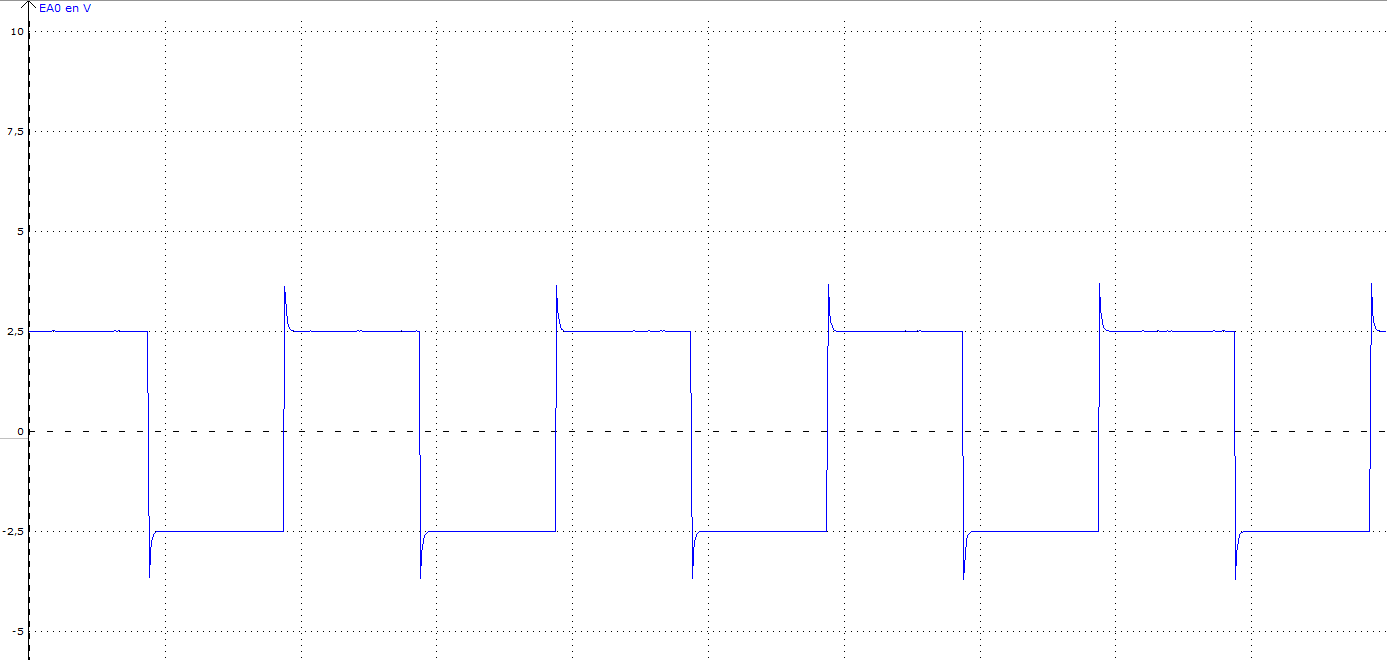
\includegraphics[scale = 0.35]{signal-0.png}\\
\noindent \underline{1-2} \\
On a \(f_e = \frac{1}{T_e} = 200kHz > 2\times f_0\)\\
Il convient donc.\\

\noindent \underline{2}
On a \begin{align*}
    \underline{H} &= \frac{H_0}{1 + jRC\omega}\\
    &= \frac{x(t)}{y(t)}\\
    \text{On pose } \tau = \frac{1}{RC}\\
    \frac{dy}{dt} + \frac{1}{\tau}y = \frac{H_0}{\tau}x
\end{align*}
\underline{2-1} \\
- La durée est de \(T_e = 5\mu s\)\\
- Avec la formule d'Euler \begin{equation*}
    \frac{y_{n+1}-y_n}{T_e} \simeq \frac{dy}{dt}
\end{equation*}
- On remplace les termes dans l'équation différentielle : \begin{align*}
    \text{On pose } H_0 = 1\\
    \frac{dy}{dt} + \frac{1}{\tau}y &= \frac{1}{\tau}x\\
    \frac{y_{n+1}-y_n}{T_e} + \frac{1}{\tau}y_n &= \frac{1}{\tau}x_n\\
    y_{n+1} &= \frac{T_e}{\tau}x_n - \frac{T_e}{\tau}y_n + y_n\\
    &= \frac{T_e}{\tau}x_n + y_n(1-\frac{T_e}{\tau})\\
    y_{n+1} &= \frac{1}{1 + \frac{\tau}{T_e}-1}(x_n + y_n(\frac{\tau}{T_e}-1))
\end{align*}
On a \(\alpha = \frac{\tau}{T_e}-1 = 19\)\\

\noindent\underline{2.2}\\
- \(y_0 = 0\) : condensateur déchargé donc il n'y a aucun courant\\
- Les 2 lignes sont équivalentes à : initialiser la valeur de \(y_0\), puis calculer \(y_{n+1}\)\\
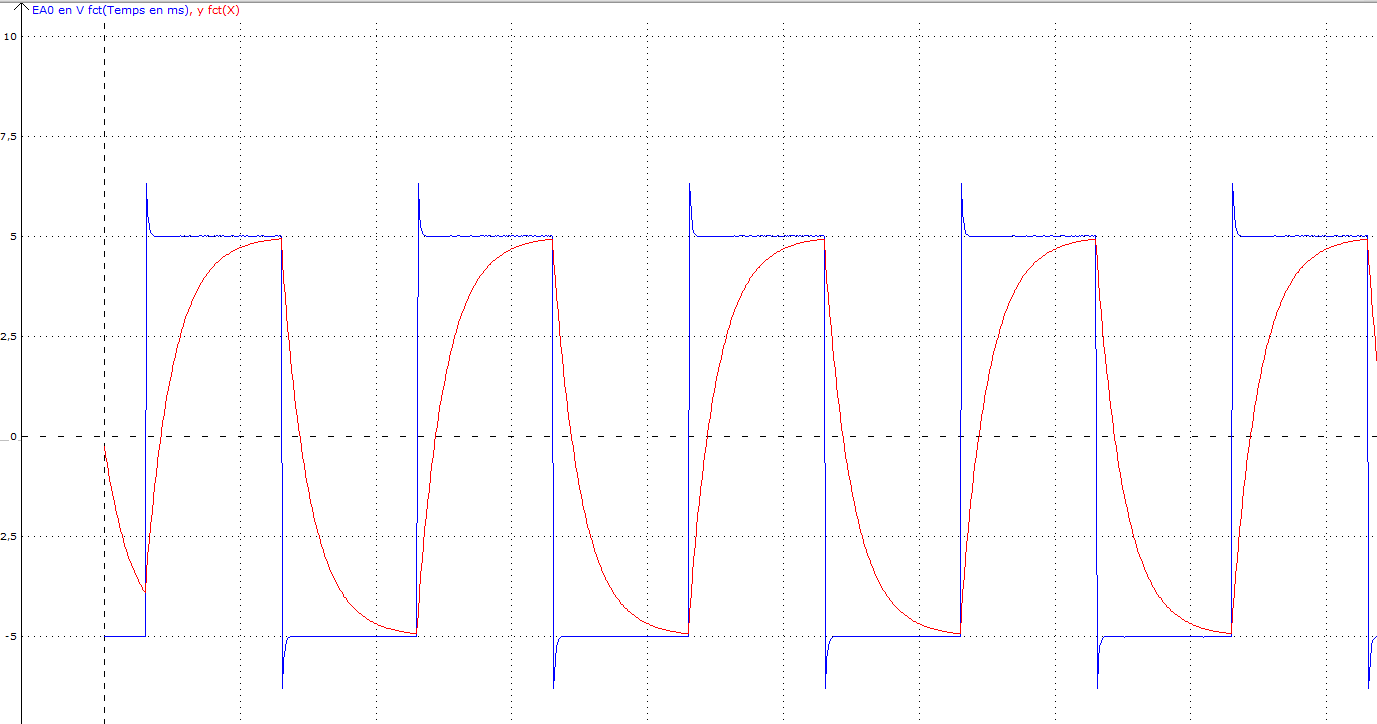
\includegraphics[scale=0.4]{signal-1.png}\\

\noindent \underline{2.4} \\
\(\Delta = 0\\
\tau = 103.56 \times 10^{-6}\\
V_0 = 5.013\)\\
\(\tau\) diffère de sa valeur théorique de \(\frac{10^{-4}}{103.56 \times 10^{-6}} = 0.97\)\\
\noindent
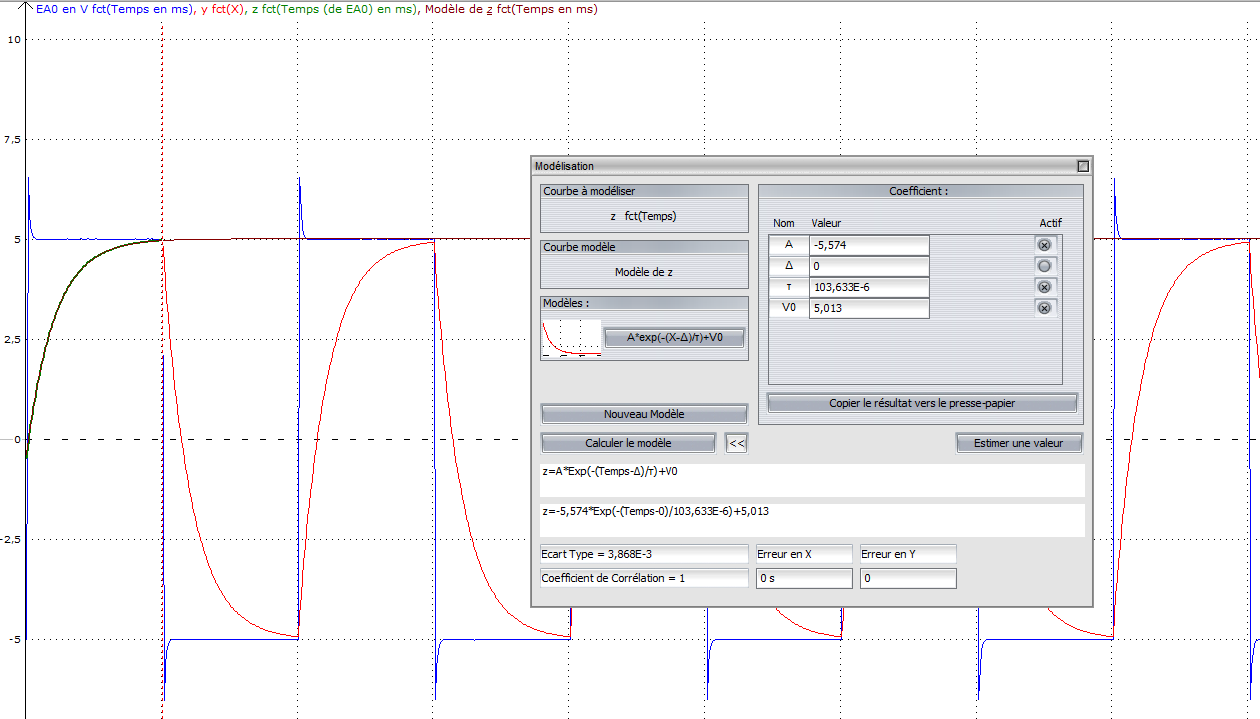
\includegraphics[scale=0.4]{modele-z.png}\\
\noindent
\underline{Spectre de y(t)}\\
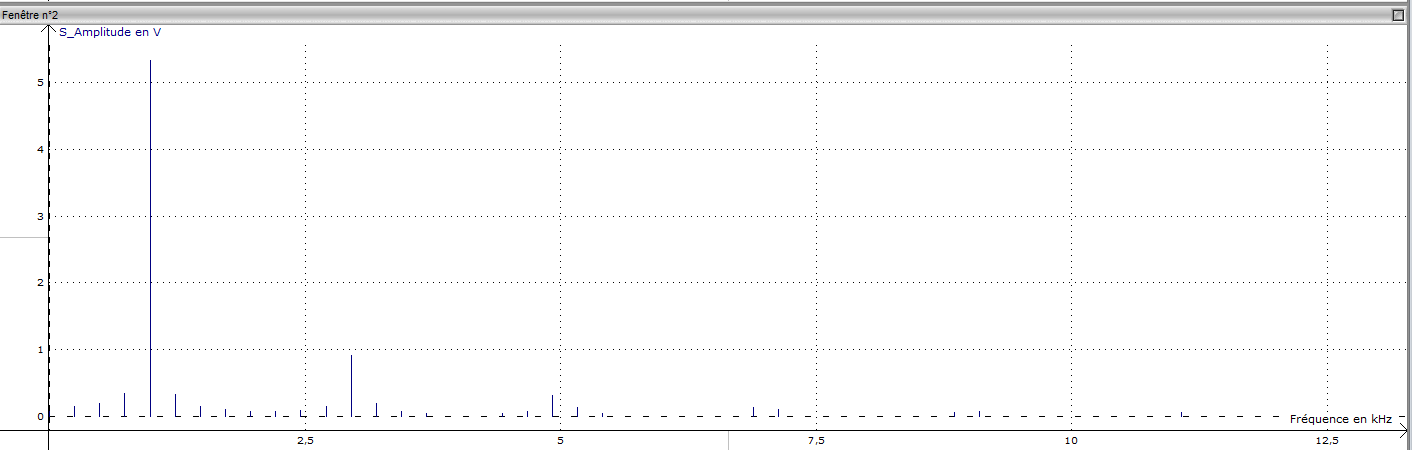
\includegraphics[scale=0.4]{spectre-y.png}

\end{document}